\section{Appendix} % o \appendix a seconda del template che stai usando

\subsection{Euler Integration Method}
\label{sec:euler_appendix}

The Euler Integration Method is a first-order numerical procedure for solving ordinary differential equations (ODEs) with a given initial value.
Being a first-order method, the local error (error per step) is proportional to the square of the step size, and the global error (error at a given time) is proportional to the step size.

\subsubsection{How it works}

Consider the problem of calculating the shape of an unknown continuous curve $y(t)$ which starts at a given initial point $y(t_0) = y_0$ and satisfies a given differential equation of the form:
\begin{equation}
    \dot{y}(t) = f(t, y(t))
\end{equation}
The function $f(t, y(t))$ can be thought of as a formula that provides the slope of the tangent line to the curve at any computed point. 

While the exact analytical expression of the curve is initially unknown, its starting point $A_0 = (t_0, y_0)$ is known. Using the differential equation, we can compute the slope of the tangent line at $A_0$. 
If we take a sufficiently small time step forward, denoted by $\Delta t$, the slope of the true curve does not change significantly. Therefore, we can move along the straight tangent line to find the next point $A_1 = (t_1, y_1)$, where $t_1 = t_0 + \Delta t$. 

Assuming the new point $A_1$ is still an acceptable approximation of the true curve, we can repeat the same reasoning: we compute the new slope at $A_1$, take another small step $\Delta t$ along the new tangent line, and find $A_2$. 

\begin{wrapfigure}{l}{0.4\textwidth}
  \centering
  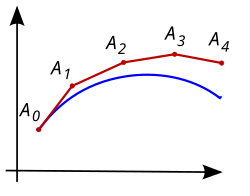
\includegraphics[width=0.38\textwidth]{Images/Euler_method.png}
  \caption{Didascalia}
\end{wrapfigure}

After several iterations, this process generates a polygonal curve $(A_0, A_1, A_2, \dots)$ that approximates the original unknown function. Mathematically, the forward projection rule at each discrete step $k$ is expressed as:
\begin{equation}
    y_{k+1} = y_k + \Delta t \cdot f(t_k, y_k)
\end{equation}
where $y_{k+1}$ is the estimated value at time $t_{k+1} = t_k + \Delta t$. In general, this polygonal curve does not diverge too far from the exact solution, and the integration error can be minimized by choosing a suitably small step size $\Delta t$.

\subsubsection{Application to Robotic Kinematics}

In the context of the \textit{local methods} for redundancy resolution discussed in the main text, the Euler method bridges the gap between differential kinematics and actual joint positions. 

At each control cycle, the optimization algorithm provides the optimal joint velocities $\dot{\mathbf{q}}(t_k)$ based on the current state. In this scenario, our ODE is simply $\dot{\mathbf{q}} = f(t, \mathbf{q})$. By applying the Euler integration step using the controller's sampling time $T_s$ as the step size, the low-level controller can compute the reference joint positions to be sent to the motors for the next instant:
\begin{equation}
    \mathbf{q}((k+1)T_s) = \mathbf{q}(kT_s) + T_s \dot{\mathbf{q}}(kT_s)
\end{equation}
This straightforward projection allows the robotic system to seamlessly execute the computed velocities in real time.

\subsection{Moore-Penrose Pseudoinverse Properties}
\label{sec:Pseudoinverse}

For any matrix $J \in \mathbb{R}^{m \times n}$, there exists a unique matrix $J^\# \in \mathbb{R}^{n \times m}$ called the Moore-Penrose pseudoinverse, which satisfies the four Penrose conditions:
\begin{enumerate}
    \item $J J^\# J = J$ \quad (generalized inverse condition)
    \item $J^\# J J^\# = J^\#$
    \item $(J J^\#)^T = J J^\#$ \quad (symmetry)
    \item $(J^\# J)^T = J^\# J$ \quad (symmetry)
\end{enumerate}

\subsubsection{Proof of the Minimum Norm Property}
Given the kinematic constraint $J\dot{\mathbf{q}} = \dot{\mathbf{y}}$, the pseudoinverse solution $\dot{\mathbf{q}}_{PS} = J^\#\dot{\mathbf{y}}$ provides the velocity vector that minimizes the Euclidean norm $\|\dot{\mathbf{q}}\|^2$ among all possible exact solutions.

\textbf{Proof:} Let $\dot{\mathbf{q}}^*$ be any generic solution that successfully realizes the task ($J\dot{\mathbf{q}}^* = \dot{\mathbf{y}}$). We must prove that $\|\dot{\mathbf{q}}^*\|^2 \ge \|\dot{\mathbf{q}}_{PS}\|^2$.
Since both solutions achieve the same task velocity:
\begin{equation}
    J\dot{\mathbf{q}}^* - J\dot{\mathbf{q}}_{PS} = \mathbf{0} \implies J(\dot{\mathbf{q}}^* - \dot{\mathbf{q}}_{PS}) = \mathbf{0}
\end{equation}
This implies that the difference vector $(\dot{\mathbf{q}}^* - \dot{\mathbf{q}}_{PS})$ belongs to the null space of the Jacobian, $\mathcal{N}(J)$. We now check if $(\dot{\mathbf{q}}^* - \dot{\mathbf{q}}_{PS})$ is orthogonal to $\dot{\mathbf{q}}_{PS}$ by computing their inner product:
\begin{align}
    (\dot{\mathbf{q}}^* - \dot{\mathbf{q}}_{PS})^T \dot{\mathbf{q}}_{PS} &= (\dot{\mathbf{q}}^* - \dot{\mathbf{q}}_{PS})^T J^T (J J^T)^{-1} \dot{\mathbf{y}} \\
    &= \left[ J (\dot{\mathbf{q}}^* - \dot{\mathbf{q}}_{PS}) \right]^T (J J^T)^{-1} \dot{\mathbf{y}} = \mathbf{0}^T (J J^T)^{-1} \dot{\mathbf{y}} = 0
\end{align}
Since they are orthogonal, we apply the Pythagorean theorem:
\begin{equation}
    \|\dot{\mathbf{q}}^*\|^2 = \|\dot{\mathbf{q}}_{PS} + (\dot{\mathbf{q}}^* - \dot{\mathbf{q}}_{PS})\|^2 = \|\dot{\mathbf{q}}_{PS}\|^2 + \|\dot{\mathbf{q}}^* - \dot{\mathbf{q}}_{PS}\|^2
\end{equation}
Since the squared norm is always non-negative ($\|\dot{\mathbf{q}}^* - \dot{\mathbf{q}}_{PS}\|^2 \ge 0$), it strictly follows that:
\begin{equation}
    \|\dot{\mathbf{q}}^*\|^2 \ge \|\dot{\mathbf{q}}_{PS}\|^2 \quad \blacksquare
\end{equation}

\subsection{Singular Value Decomposition (SVD)}
\label{sec:SVD}

To compute the pseudoinverse robustly, especially when $J$ loses rank, the \textbf{Singular Value Decomposition} is used. 
Every Jacobian matrix $J$ can be decomposed as $J = U \Sigma V^T$, where $U \in \mathbb{R}^{m \times m}$ and $V \in \mathbb{R}^{n \times n}$ 
are orthogonal matrices, and $\Sigma \in \mathbb{R}^{m \times n}$ is a diagonal matrix containing the singular values $\sigma_i$ on its main diagonal.

The pseudoinverse is computed as:
\begin{equation}
    J^\# = V \Sigma^\# U^T
\end{equation}
where $\Sigma^\#$ is obtained by transposing $\Sigma$ 
and replacing every non-zero singular value $\sigma_i$ with its reciprocal $1/\sigma_i$. 
Zero singular values are left as zero, safely avoiding division by zero at exact singularities.

\subsection{Damped Least Squares (DLS)}
\label{sec:DLS}

While SVD handles exact singularities, algorithmic instability occurs in the \textit{neighborhood} of a 
singularity, where a singular value $\sigma_i \approx 0$. Its reciprocal $1/\sigma_i \to \infty$ generates explosive joint velocities.

The \textbf{Damped Least Squares} method achieves singularity robustness by relaxing the exact tracking 
constraint $J\dot{\mathbf{q}} = \dot{\mathbf{y}}$. It formulates an unconstrained optimization problem that 
balances the task tracking error and the joint velocity norm using a damping factor $\mu^2 > 0$:
\begin{equation}
    \min_{\dot{\mathbf{q}}} \left( \frac{1}{2} \|\dot{\mathbf{y}} - J\dot{\mathbf{q}}\|^2 + \frac{\mu^2}{2} \|\dot{\mathbf{q}}\|^2 \right)
\end{equation}
Setting the gradient with respect to $\dot{\mathbf{q}}$ to zero yields the analytical DLS solution:
\begin{equation}
    \dot{\mathbf{q}}_{DLS} = J^T(J J^T + \mu^2 I_m)^{-1} \dot{\mathbf{y}}
\end{equation}
The addition of $\mu^2 I_m$ guarantees that the matrix $(J J^T + \mu^2 I_m)$ is 
strictly positive definite and invertible everywhere. When far from singularities, 
$\mu \to 0$ and the solution converges to the pseudoinverse. Near singularities, $\mu$ dominates, 
smoothly capping the joint velocities at the cost of a small, allowable task tracking error.